\chapter{Arbres phylogénétiques et horloge moléculaire}\label{ch:b2:phylogenetic-trees}

En 1965, deux chimistes, Emile Zuckerkandl et Linus Pauling, comparèrent
les séquences d'acides aminés de l'hémoglobine d'une poignée de
vertébrés et remarquèrent ce qu'aucun anatomiste n'aurait pu voir~: le
nombre de différences entre deux espèces était proportionnel au temps
écoulé depuis la séparation de leurs ancêtres, tel que le révèlent les
fossiles. Une molécule mesurait le temps. En moins de dix ans, Carl Woese
utilisa un seul gène, l'ARN de la petite sous-unité du ribosome, pour
dessiner l'arbre de tout le vivant et y découvrir un troisième domaine,
les archées, qu'aucun microscope n'avait distinguées des bactéries. Ce
chapitre traite de la reconstruction de l'histoire à partir de la
ressemblance~: ce que signifie un arbre, comment on le construit à partir
de caractères et de distances, comment on fait dire le temps aux
séquences, et les pièges --- convergence, vitesses inégales, saturation,
longues branches --- que doit connaître tout lecteur d'arbres.

\section{Lire un arbre}

\begin{definition}[Phylogénie, clade, homologie]\label{def:b2:phylogenetic-trees:tree}
\index{phylogenie@phylogénie}\index{clade}\index{groupe monophyletique@groupe monophylétique}\index{groupe paraphyletique@groupe paraphylétique}\index{groupe polyphyletique@groupe polyphylétique}\index{homologie}\index{analogie}\index{synapomorphie}
Une \emph{phylogénie} est un arbre dont les extrémités sont les espèces
(ou les gènes, ou les individus) comparées, dont les nœuds internes sont
leurs ancêtres communs, et dont la racine est l'ancêtre le plus ancien de
tous. Son ordre de branchement porte à lui seul l'histoire~: on peut faire
pivoter librement les nœuds, seul l'emboîtement compte. Un \emph{clade} ou
\emph{groupe monophylétique} est un ancêtre avec \emph{tous} ses
descendants (les oiseaux~; les mammifères~; les oiseaux et les crocodiles
ensemble)~; un groupe \emph{paraphylétique} est un ancêtre dont certains
descendants sont laissés de côté («~reptiles~» sans les oiseaux,
«~poissons~» sans les tétrapodes, «~\omterm{def:b2:unicellular-diversity:prokaryote}{procaryotes}~»)~; un groupe
\emph{polyphylétique} réunit des descendants d'ancêtres différents par
une ressemblance acquise séparément («~animaux à sang chaud~»). Un
caractère partagé par deux espèces parce que leur ancêtre le possédait
est une \emph{homologie} (les os de l'aile de la chauve-souris et de la
nageoire de la baleine)~; un caractère acquis indépendamment est une
\emph{analogie} ou \emph{homoplasie} (les ailes des chauves-souris et des
oiseaux en tant qu'ailes, les yeux en chambre noire des vertébrés et des
pieuvres). Seules les homologies enregistrent l'histoire, et parmi elles
seuls les états \emph{dérivés} partagés par un groupe --- ses
\emph{synapomorphies}, selon le mot de Hennig --- définissent un clade~:
les plumes définissent les oiseaux, l'état ancestral «~pas de plumes~» ne
définit rien.
\end{definition}

\begin{omfigure}
\begin{tikzpicture}[every node/.style={font=\scriptsize}, >=stealth, line width=0.8pt]
  \coordinate (root) at (0,0);
  \coordinate (n1) at (1.2,0.9); \coordinate (n2) at (2.4,1.6); \coordinate (n3) at (3.6,2.3);
  \draw (root) -- (1.4,-1.3) node[right] {mammifères};
  \draw (root) -- (n1);
  \draw (n1) -- (4.8,-0.1) node[right] {tortues};
  \draw (n1) -- (n2);
  \draw (n2) -- (4.8,0.9) node[right] {lézards, serpents};
  \draw (n2) -- (n3);
  \draw (n3) -- (4.8,1.9) node[right] {crocodiles};
  \draw (n3) -- (4.8,3.0) node[right] {oiseaux};
  \fill (root) circle (1.6pt); \fill (n1) circle (1.6pt); \fill (n2) circle (1.6pt); \fill (n3) circle (1.6pt);
  \node[left] at (root) {amniotes};
  % groups
  \draw[omThm, thick, rounded corners=6pt] (3.1,1.55) rectangle (6.9,3.4);
  \node[omThm, anchor=south west] at (3.1,3.4) {archosaures~: monophylétique};
  \draw[omExo!80!black, thick, dashed, rounded corners=6pt] (2.2,-0.5) -- (2.2,2.2) -- (7.1,2.2) -- (7.1,-0.5) -- cycle;
  \node[omExo!80!black, anchor=north east] at (7.1,-0.55) {«~reptiles~» sans les oiseaux~: paraphylétique};
  \node[anchor=west, align=left, text width=4.2cm] at (7.9,1.3) {synapomorphies~:\\ $\bullet$ œuf amniotique (tous)\\ $\bullet$ fenêtre antéorbitaire du crâne (archosaures)\\ $\bullet$ plumes (oiseaux)};
\end{tikzpicture}

{\small Lire un arbre. Les oiseaux s'emboîtent dans les reptiles~: les
crocodiles sont plus proches des oiseaux que des lézards. Le groupe nommé
«~reptiles~» est un ancêtre dont une lignée de descendants a été retirée
--- un grade paraphylétique, non un \omterm{def:b2:phylogenetic-trees:tree}{clade}.}
\end{omfigure}

\begin{omfigure}
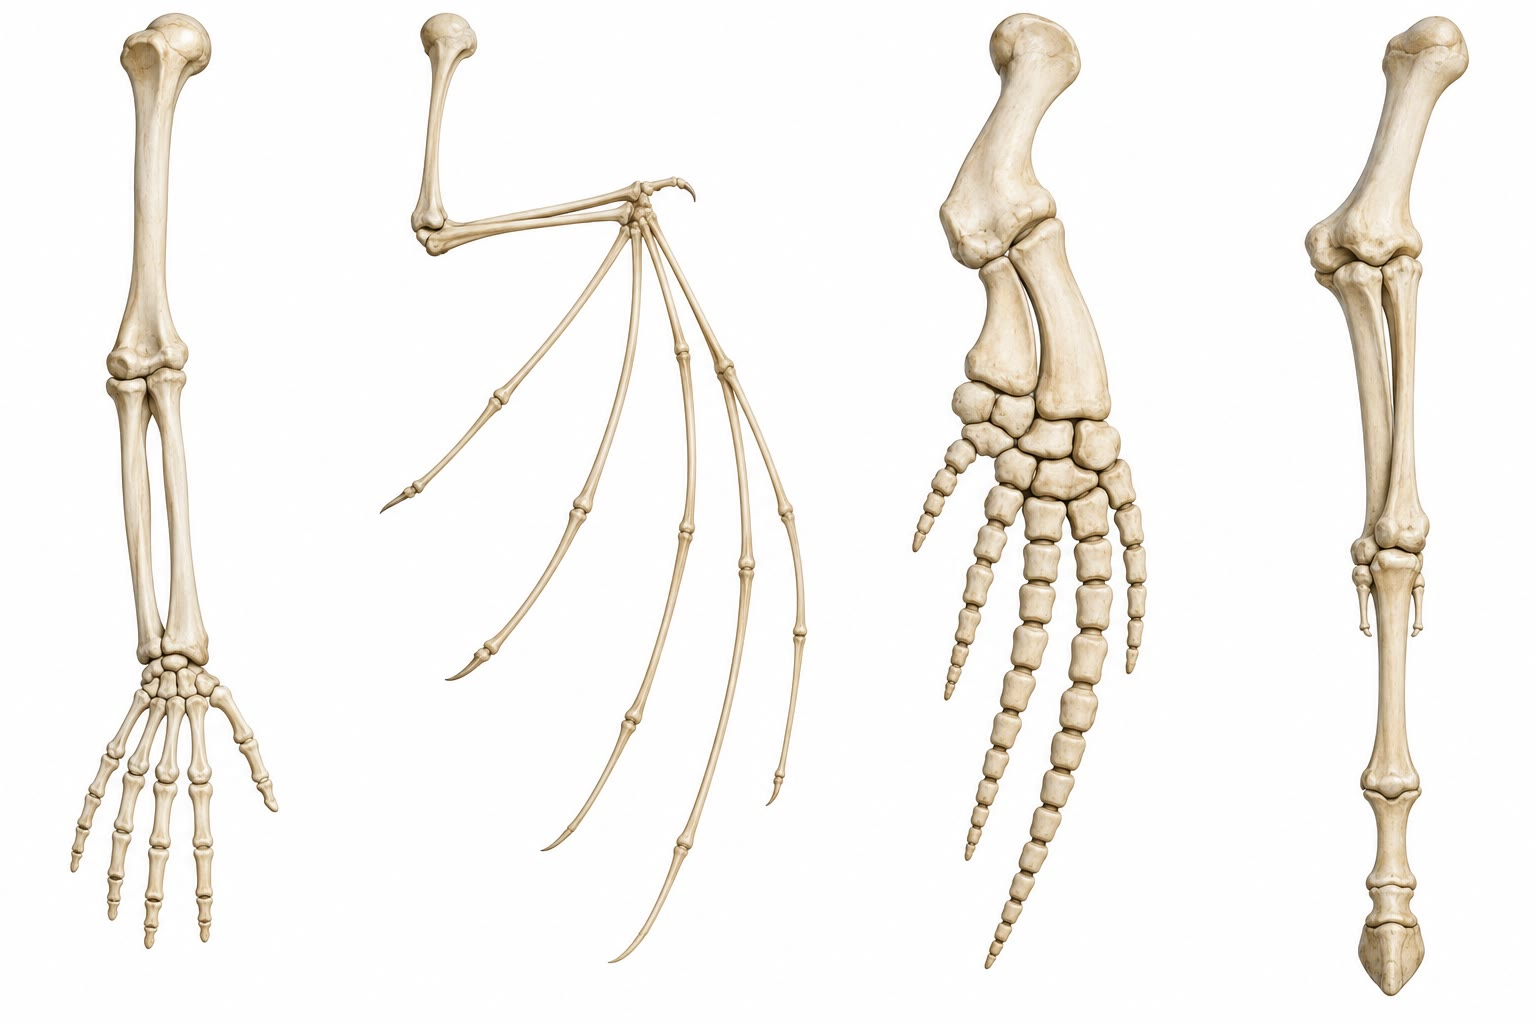
\includegraphics[width=0.44\linewidth]{images/book4/ai/b4-24-homologous-forelimbs.jpg}\hspace{0.04\linewidth}
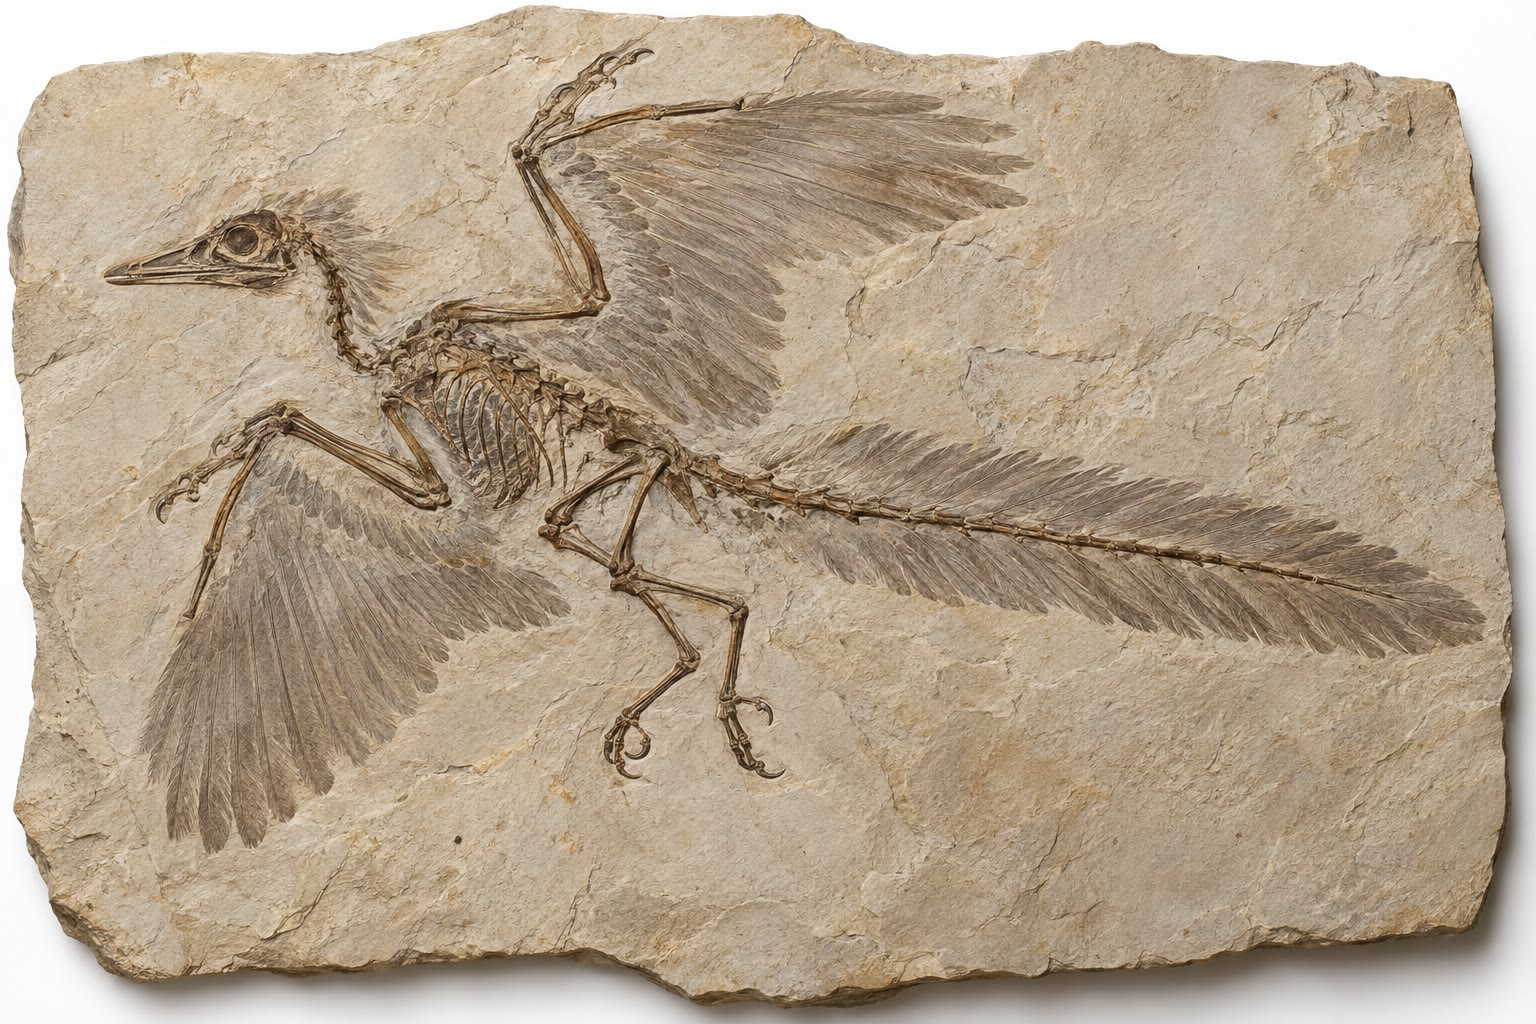
\includegraphics[width=0.44\linewidth]{images/book4/ai/b4-24-archaeopteryx.jpg}

{\small L'\omterm{def:b2:phylogenetic-trees:tree}{homologie} et ses traces. À gauche~: les mêmes os --- humérus,
radius et ulna, poignet, cinq doigts --- dans un bras, une aile, une
nageoire et une patte. À droite~: \emph{Archaeopteryx}, avec les dents,
les doigts griffus et la longue queue osseuse d'un petit dinosaure et
les plumes d'un oiseau.}
\end{omfigure}

\section{Construire des arbres à partir de caractères}

\begin{method}[La parcimonie]\label{meth:b2:phylogenetic-trees:parsimony}
\index{parcimonie}\index{groupe externe}\index{bootstrap}
Coder les caractères (états morphologiques ou positions de séquences
alignées) pour chaque taxon. Pour chaque arbre possible, compter le
nombre minimal de changements de caractères nécessaires pour y expliquer
les données~; l'arbre le plus parcimonieux en demande le moins. Enraciner
l'arbre au moyen d'un
\emph{\omterm{meth:b2:phylogenetic-trees:parsimony}{groupe externe}}, un taxon dont on sait qu'il se situe hors du groupe
étudié. Comme le nombre d'arbres non enracinés pour $n$ taxons vaut $1\cdot 3\cdot
5\cdots(2n - 5)$ --- trois pour quatre taxons, $2\times 10^{6}$ pour dix,
$10^{20}$ pour vingt --- la recherche n'est exhaustive que pour de petits
ensembles et heuristique au-delà. La confiance se mesure par le
\emph{bootstrap}~: rééchantillonner les caractères avec remise un millier
de fois, reconstruire l'arbre à chaque fois, et noter la fréquence à
laquelle chaque \omterm{def:b2:phylogenetic-trees:tree}{clade} réapparaît~; un \omterm{def:b2:phylogenetic-trees:tree}{clade} retrouvé dans \qty{95}{\%} des
rééchantillonnages est bien soutenu, un \omterm{def:b2:phylogenetic-trees:tree}{clade} retrouvé dans la moitié ne
l'est pas.
\end{method}

\begin{example}[Quatre taxons, cinq sites]\label{ex:b2:phylogenetic-trees:parsimony}
Séquences $A = \mathrm{AAGCT}$, $B = \mathrm{AAGCC}$, $C =
\mathrm{GGACT}$, $D = \mathrm{GGATC}$. Sur l'arbre $((A,B),(C,D))$,
les sites 1, 2 et 3 changent chacun une fois (sur la branche interne), le
site 4 une fois ($\mathrm{C}\to\mathrm{T}$ chez $D$) et le site 5 deux fois
($\mathrm{T}\to\mathrm{C}$ chez $B$ et chez $D$)~: six pas. Sur
$((A,C),(B,D))$, les sites 1 à 3 demandent chacun deux changements, les
sites 4 et 5 un chacun~: huit. Sur $((A,D),(B,C))$~: neuf. Le premier arbre
est le plus parcimonieux, avec deux pas d'avance~; les trois sites qui le
soutiennent sont ses \omterm{def:b2:phylogenetic-trees:tree}{synapomorphies}, et le site 5 est une homoplasie sur
cet arbre --- le même changement survenu deux fois, une réalité de tout
jeu de données réel.
\end{example}

\begin{omfigure}
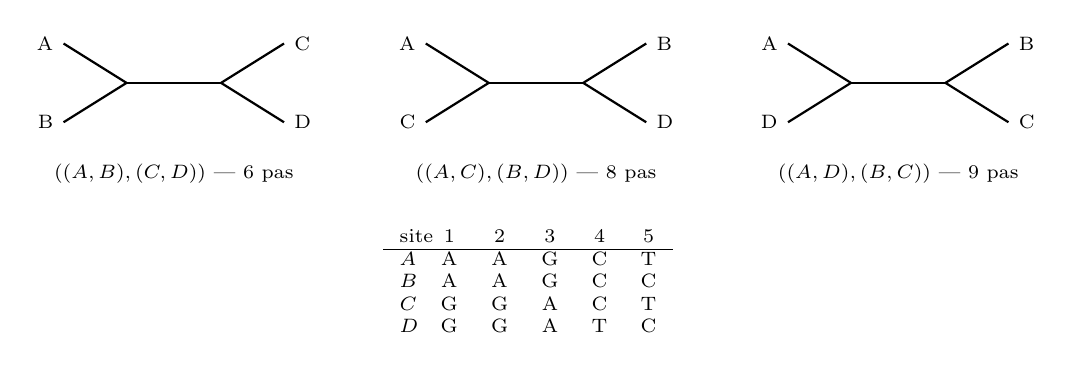
\begin{tikzpicture}[every node/.style={font=\scriptsize}, line width=0.8pt]
  \foreach \x/\a/\b/\c/\d/\steps/\lab in {0/A/B/C/D/6/{$((A,B),(C,D))$ --- 6 pas}, 4.6/A/C/B/D/8/{$((A,C),(B,D))$ --- 8 pas}, 9.2/A/D/B/C/9/{$((A,D),(B,C))$ --- 9 pas}} {
    \begin{scope}[xshift=\x cm]
      \draw (0,1.6) node[left] {\a} -- (0.8,1.1) -- (0,0.6) node[left] {\b};
      \draw (0.8,1.1) -- (2.0,1.1);
      \draw (2.8,1.6) node[right] {\c} -- (2.0,1.1) -- (2.8,0.6) node[right] {\d};
      \node[anchor=north] at (1.4,0.2) {\lab};
    \end{scope}
  }
  \node[anchor=north] at (5.9,-0.6) {\begin{tabular}{l@{\ }ccccc} site & 1 & 2 & 3 & 4 & 5 \\ \hline $A$ & A & A & G & C & T \\ $B$ & A & A & G & C & C \\ $C$ & G & G & A & C & T \\ $D$ & G & G & A & T & C \end{tabular}};
\end{tikzpicture}

{\small Les trois arbres non enracinés pour quatre taxons, évalués sur
l'alignement de cinq sites placé en dessous. Les sites 1 à 3 changent une
fois sur le premier arbre et deux fois sur les autres~; le site 4 ne varie
que chez un seul taxon et ne peut pas trancher, tandis que le site 5
regroupe $A$ avec $C$ et favorise donc le troisième arbre contre eux.}
\end{omfigure}

\section{Construire des arbres à partir de distances}

\begin{method}[Regroupement par distance~: UPGMA]\label{meth:b2:phylogenetic-trees:upgma}
\index{UPGMA}\index{agregation des voisins@agrégation des voisins}\index{matrice des distances}
À partir des distances deux à deux entre $n$ taxons (différences par site,
corrigées comme ci-dessous), réunir la paire la plus proche en un groupe
placé en un nœud de hauteur égale à la moitié de leur distance~; remplacer
la paire par le groupe, dont la distance à chaque autre taxon est la
moyenne des distances de ses membres~; recommencer jusqu'à ce qu'il ne
reste qu'un groupe. Le résultat
est un arbre enraciné dont toutes les extrémités sont à la même hauteur
--- il suppose une vitesse de changement constante sur chaque branche,
une \omterm{thm:b2:phylogenetic-trees:clock}{horloge moléculaire}. Lorsque les vitesses diffèrent entre lignées, la
méthode regroupe les lignées à évolution rapide, quelle que soit leur
histoire~; l'\emph{\omterm{meth:b2:phylogenetic-trees:upgma}{agrégation des voisins}} (neighbour joining),
qui réunit à chaque étape la paire dont l'union raccourcit le plus
l'arbre entier, ne suppose pas d'horloge et constitue la méthode rapide
standard pour les grands jeux de données.
\end{method}

\begin{example}[UPGMA]\label{ex:b2:phylogenetic-trees:upgma}
Distances (en différences pour cent sites)~: $AB = 4$, $AC = 8$,
$AD = 10$, $BC = 8$, $BD = 10$, $CD = 6$. Réunir $A$ et $B$ à la hauteur 2~;
puis $d(AB, C) = 8$, $d(AB, D) = 10$, $d(C,D) = 6$~: réunir $C$ et $D$ à
la hauteur 3~; enfin $d(AB, CD) = (8 + 10 + 8 + 10)/4 = 9$~: réunir les
deux groupes à la hauteur $4.5$. L'arbre est $((A,B),(C,D))$, et si
la vitesse est de $10^{-9}$ substitution par site et par an, la racine a
$0.045/10^{-9} = 45$ millions d'années.
\end{example}

\begin{omfigure}
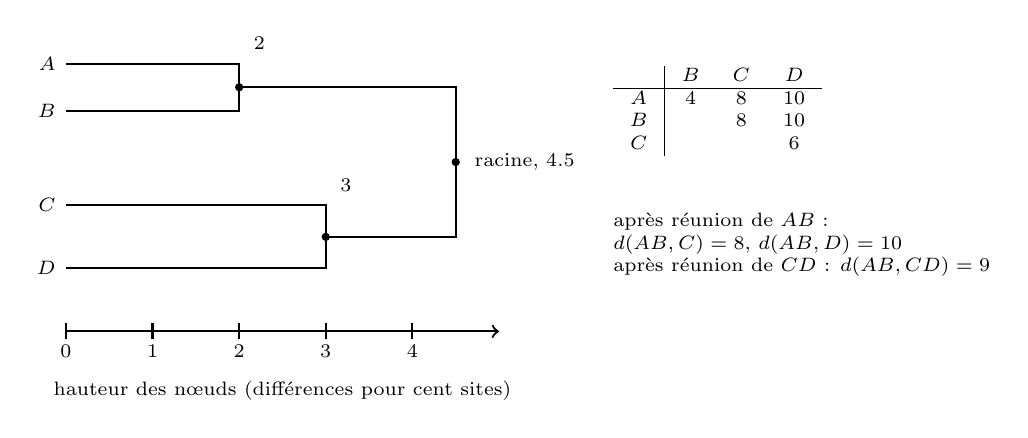
\begin{tikzpicture}[every node/.style={font=\scriptsize}, line width=0.8pt, x=1.1cm]
  \draw[->] (0,-0.4) -- (5,-0.4); \foreach \h in {0,1,2,3,4} \draw (\h,-0.5) -- (\h,-0.3) node[below=4pt] {\h};
  \node[anchor=north] at (2.5,-0.9) {hauteur des nœuds (différences pour cent sites)};
  % A,B join at 2, C,D at 3, root at 4.5 ; draw as rooted tree, root on the right
  \draw (0,3.0) node[left] {$A$} -- (2,3.0) -- (2,2.4) -- (0,2.4) node[left] {$B$};
  \draw (0,1.2) node[left] {$C$} -- (3,1.2) -- (3,0.4) -- (0,0.4) node[left] {$D$};
  \draw (2,2.7) -- (4.5,2.7) -- (4.5,0.8) -- (3,0.8);
  \fill (2,2.7) circle (1.5pt); \fill (3,0.8) circle (1.5pt); \fill (4.5,1.75) circle (1.5pt);
  \node[anchor=west] at (4.6,1.75) {racine, 4.5};
  \node[anchor=south west] at (2.05,3.05) {2};
  \node[anchor=south west] at (3.05,1.25) {3};
  \node[anchor=west, align=left] at (6.2,2.4) {\begin{tabular}{c|ccc} & $B$ & $C$ & $D$ \\ \hline $A$ & 4 & 8 & 10 \\ $B$ & & 8 & 10 \\ $C$ & & & 6 \end{tabular}};
  \node[anchor=west, align=left] at (6.2,0.7) {après réunion de $AB$~:\\ $d(AB,C) = 8$, $d(AB,D) = 10$\\ après réunion de $CD$~: $d(AB,CD) = 9$};
\end{tikzpicture}

{\small UPGMA sur quatre taxons. Chaque nœud se situe à la moitié de la
distance entre les groupes qu'il réunit~; toutes les extrémités se
terminent à la hauteur zéro, comme l'exige une horloge.}
\end{omfigure}

\section{L'horloge moléculaire}

\begin{theorem}[Les substitutions comme processus de Poisson, et la correction des substitutions multiples]\label{thm:b2:phylogenetic-trees:clock}
\index{horloge moleculaire@horloge moléculaire}\index{correction de Jukes--Cantor}\index{saturation}
Si les substitutions en un site surviennent à une vitesse constante $k$
par an, indépendamment d'un site à l'autre, le nombre de substitutions
qui s'accumulent le long d'une lignée en un temps $t$ suit une loi de
Poisson de moyenne $kt$, et le nombre attendu de substitutions qui
séparent deux lignées ayant divergé il y a $t$ années vaut
\[
d = 2kt
\]
substitutions par site --- l'\emph{\omterm{thm:b2:phylogenetic-trees:clock}{horloge moléculaire}}. La proportion
observée $p$ de sites qui diffèrent est inférieure à $d$, car un
site touché deux fois peut revenir à sa base d'origine ou coïncider par
hasard~; avec quatre bases changeant à des vitesses égales,
\[
p = \tfrac{3}{4}\bigl(1 - e^{-4d/3}\bigr), \qquad
d = -\tfrac{3}{4}\ln\bigl(1 - \tfrac{4}{3}p\bigr),
\]
la correction de \emph{Jukes--Cantor}. Quand $d$ augmente, $p$ sature à
$3/4$ --- deux séquences aléatoires coïncident en un quart de leurs sites
--- et au-delà de $p \approx 0.5$ la correction amplifie toute erreur
d'échantillonnage~: un gène qui a autant changé ne mesure plus le temps.
Les gènes lents (ARN ribosomique, histones) datent les branches
profondes, les gènes rapides (ADN mitochondrial, introns) les branches
récentes.
\end{theorem}
\begin{proof}
Soit $q(t)$ la probabilité qu'un site porte encore sa base d'origine
après un temps $t$. Elle est perdue à la vitesse $k$ et regagnée, à partir
de chacune des trois autres bases, à la vitesse $k/3$~:
$\mathrm{d}q/\mathrm{d}t = -kq + \tfrac{k}{3}(1 - q) = \tfrac{k}{3} -
\tfrac{4k}{3}q$, dont la solution avec $q(0) = 1$ est $q = \tfrac14 +
\tfrac34 e^{-4kt/3}$. Deux lignées séparées par un temps total $2t$ ---
par symétrie, comme une seule lignée évoluant pendant $2t$ --- coïncident
en un site avec la probabilité $\tfrac14 + \tfrac34 e^{-4d/3}$ où $d =
2kt$, donc $p = 1 - q = \tfrac34(1 - e^{-4d/3})$~; l'inversion donne la
correction. Le comptage de Poisson découle d'événements constants et
indépendants, comme en physique de la désintégration radioactive, et son
écart-type $\sqrt{kt}$ fixe la précision de toute date~: un gène de $L$
sites présentant $dL$ substitutions observées date une divergence avec
une précision relative d'environ $1/\sqrt{dL}$.
\end{proof}
\begin{proof}[Faits expérimentaux]
Zuckerkandl et Pauling (1965) trouvèrent les différences entre les
hémoglobines du cheval, de l'homme, de la vache et d'autres espèces
proportionnelles aux âges fossiles de leurs séparations, et proposèrent
l'horloge. Fitch et
Margoliash (1967) construisirent un arbre de vingt espèces à partir du seul
cytochrome $c$ et retrouvèrent, à partir d'une seule protéine, les
regroupements classiques des vertébrés, des insectes et des champignons.
Le test décisif de la méthode fut la \omterm{def:b2:phylogenetic-trees:tree}{phylogénie} expérimentale de Hillis et
de ses collègues (1992)~: ils propagèrent le bactériophage T7 selon une
série connue et ramifiée de huit lignées sous l'effet d'un mutagène,
séquencèrent les produits et soumirent les séquences en aveugle aux
méthodes de construction d'arbres --- les méthodes de parcimonie, de
distance et de vraisemblance retrouvèrent toutes le véritable arbre, et
la parcimonie reconstitua les séquences ancestrales avec plus de
\qty{98}{\%} d'exactitude.
\end{proof}

\begin{omfigure}
\begin{tikzpicture}
\begin{axis}[
  width=0.7\linewidth, height=5.4cm,
  axis x line=bottom, axis y line=left,
  xmin=0, xmax=2.5, ymin=0, ymax=1.05,
  xlabel={substitutions réelles par site, $d$}, ylabel={différences observées, $p$},
  xlabel style={font=\small, at={(axis description cs:0.5,-0.13)}, anchor=north},
  ylabel style={font=\small},
  tick label style={font=\small}, ytick={0,0.25,0.5,0.75,1},
  legend style={font=\scriptsize, at={(0.97,0.35)}, anchor=east, draw=none},
  clip=false,
]
\addplot[very thick, omDef, domain=0:2.5, samples=80] {0.75*(1-exp(-4*x/3))};
\addlegendentry{$p = \tfrac34(1 - e^{-4d/3})$}
\addplot[thick, gray, dashed, domain=0:1.05, samples=2] {x};
\addlegendentry{$p = d$~: sans substitutions multiples}
\draw[dotted, gray] (axis cs:0,0.75) -- (axis cs:2.5,0.75); \node[font=\scriptsize, anchor=south east] at (axis cs:2.5,0.75) {saturation, $p = 3/4$};
\draw[<->, omThm, thick] (axis cs:0.383,0.30) -- (axis cs:0.383,0.383); \node[font=\scriptsize, omThm, anchor=west] at (axis cs:0.5,0.22) {$p = 0.30$ correspond à $d = 0.38$};
\end{axis}
\end{tikzpicture}

{\small Les substitutions multiples. La fraction observée de sites
différents augmente avec le nombre réel de substitutions puis sature~;
un $p$ brut sous-estime toutes les distances et comprime les branches
profondes d'un arbre.}
\end{omfigure}

\begin{proposition}[Les pièges de l'horloge et des arbres]\label{prop:b2:phylogenetic-trees:pitfalls}
\index{attraction des longues branches}\index{heterogeneite des vitesses@hétérogénéité des vitesses}\index{tri incomplet des lignees@tri incomplet des lignées}\index{vraisemblance (phylogenetique)@vraisemblance (phylogénétique)}
L'horloge n'est qu'approximativement constante~: les vitesses diffèrent
d'un facteur cent entre gènes (selon la fonction --- l'histone H4 a changé
deux résidus en un milliard d'années, les fibrinopeptides changent tous
les quelques millions d'années), entre sites d'un même gène (troisièmes
positions des codons, introns et boucles changent le plus vite), et entre
lignées (l'horloge des rongeurs bat plus vite que celle des primates,
avec leurs générations plus courtes et leur métabolisme plus intense).
Toute horloge exige donc un
\emph{étalonnage} par un fossile ou un événement géologique daté, et les
dates portent l'erreur de Poisson ci-dessus et celle de l'étalonnage.
Les arbres ont leurs propres pièges. L'\emph{\omterm{prop:b2:phylogenetic-trees:pitfalls}{attraction des longues
branches}}~: deux lignées qui ont chacune beaucoup changé partagent par
hasard de nombreux sites, et la parcimonie les réunit quelle que soit leur
histoire --- le remède est un échantillonnage plus dense, qui brise les
branches, et une méthode qui modélise les vitesses. La \emph{convergence}
produit de fausses \omterm{def:b2:phylogenetic-trees:tree}{synapomorphies}. Le \emph{\omterm{prop:b2:phylogenetic-trees:pitfalls}{tri incomplet des lignées}}~:
l'arbre d'un gène n'est pas nécessairement celui des espèces lorsque les
spéciations se succèdent rapidement, car le polymorphisme ancestral se
répartit différemment dans chaque descendant
--- c'est pourquoi un arbre d'espèces se construit à partir de nombreux
gènes, et non d'un seul. Et chez les \omterm{def:b2:unicellular-diversity:prokaryote}{procaryotes}, où les gènes se
déplacent latéralement
(\cref{ch:b2:genome-diversification}), des gènes différents racontent
des histoires différentes, et l'histoire est un réseau que traverse un
arbre des gènes ribosomiques. La pratique moderne remplace la parcimonie
et les distances par la \emph{vraisemblance}~: étant donné un modèle de
substitution (les vitesses de chaque changement, leur variation entre
sites), calculer la probabilité des séquences observées sur chaque arbre
avec ses longueurs de branches, et choisir l'arbre qui rend les données
les plus probables~; sa forme bayésienne donne directement une probabilité
pour chaque \omterm{def:b2:phylogenetic-trees:tree}{clade}. Le volume de troisième année expose ces méthodes~; il
suffit ici de savoir que tout arbre est une hypothèse assortie d'un
soutien mesuré, et non un fait.
\end{proposition}
\begin{proof}[Faits expérimentaux]
Woese et Fox (1977) comparèrent l'ARN ribosomique de la petite sous-unité
chez des \omterm{def:b2:unicellular-diversity:prokaryote}{procaryotes} et trouvèrent les méthanogènes aussi éloignés des
bactéries que les uns et les autres le sont des eucaryotes~: les trois
domaines, confirmés depuis par chaque gène de la machinerie de
transcription et de traduction, et invisibles pour la morphologie. Les
mêmes arbres ribosomiques, lus naïvement, plaçaient les microsporidies, à
évolution rapide, à la base des eucaryotes~; des gènes plus lents, et des
modèles tenant compte de la variation des vitesses, les ont déplacées
parmi les champignons, où elles ont leur place --- un cas d'école
d'\omterm{prop:b2:phylogenetic-trees:pitfalls}{attraction des longues branches} détectée et corrigée.
\end{proof}

\begin{omfigure}
\begin{tikzpicture}[every node/.style={font=\scriptsize}, line width=0.8pt]
  \node[anchor=south] at (1.5,2.6) {arbre réel};
  \draw (0,2.2) node[left] {$A$} -- (0.8,1.6) -- (0,1.0) node[left] {$B$};
  \draw (0.8,1.6) -- (1.6,1.6);
  \draw[very thick, omThm] (1.6,1.6) -- (3.4,2.4) node[right] {$C$ (rapide)};
  \draw[very thick, omThm] (0.8,1.6) -- (0.8,0.2) -- (2.6,0.2) node[right] {$D$ (rapide)};
  \draw (1.6,1.6) -- (2.4,1.0) node[right] {$E$};
  \begin{scope}[xshift=7cm]
    \node[anchor=south] at (1.5,2.6) {arbre trouvé par la parcimonie};
    \draw (0,2.2) node[left] {$A$} -- (0.8,1.6) -- (0,1.0) node[left] {$B$};
    \draw (0.8,1.6) -- (1.6,1.6);
    \draw (1.6,1.6) -- (2.4,1.9) node[right] {$E$};
    \draw[very thick, omThm] (1.6,1.6) -- (2.2,1.0) -- (3.4,1.3) node[right] {$C$};
    \draw[very thick, omThm] (2.2,1.0) -- (3.0,0.2) node[right] {$D$};
  \end{scope}
  \node[align=center, text width=7cm] at (5.6,-1.1) {$C$ et $D$ ont chacun changé en de nombreux sites~; en un quart de ceux-ci, ils coïncident désormais par hasard, plus qu'aucune vraie synapomorphie ne les relie à leurs véritables apparentés};
\end{tikzpicture}

{\small L'\omterm{prop:b2:phylogenetic-trees:pitfalls}{attraction des longues branches}. Deux lignées qui ont évolué le
plus vite sont réunies par les coïncidences fortuites que produisent
leurs nombreux changements, et la parcimonie en fait des groupes frères.}
\end{omfigure}

\begin{example}[Dater avec un fossile]\label{ex:b2:phylogenetic-trees:dating}
Un gène de \num{1000} sites diffère en \qty{10}{\%} d'entre eux entre la
vache et la baleine, dont les fossiles placent l'ancêtre commun à 60
millions d'années. Après correction, $d = -0.75\ln(1 - 0.133) = 0.107$~; la
vitesse vaut $k
= d/2t = 0.107/(1.2\times 10^{8}) = 9\times 10^{-10}$ par site et par
an. Le même gène diffère en \qty{6}{\%} des sites entre la baleine et
l'hippopotame~:
$d = 0.0625$, $t = d/2k = 35$ millions d'années, avec environ $\pm
\qty{13}{\%}$ d'après le comptage de Poisson de 62 substitutions, et une
incertitude supplémentaire due à la date fossile. Le résultat moléculaire
selon lequel les baleines sont les plus proches parents actuels des
hippopotames, obtenu ainsi dans les années 1990 contre tous les arbres
anatomiques, fut confirmé par la découverte de baleines primitives
possédant l'astragale de type hippopotame prédit --- l'horloge ne se
contente pas de dater~; elle prédit ce que les roches doivent contenir.
\end{example}

\section{Exercices}

\begin{exercise}[$\star$]\label{exo:b2:phylogenetic-trees:1}
Définir \omterm{def:b2:phylogenetic-trees:tree}{homologie}, \omterm{def:b2:phylogenetic-trees:tree}{analogie} et \omterm{def:b2:phylogenetic-trees:tree}{synapomorphie}, avec un exemple de chacune
parmi les membres, les ailes et les yeux des vertébrés.
\end{exercise}

\begin{exercise}[$\star$]\label{exo:b2:phylogenetic-trees:2}
Classer comme monophylétique, paraphylétique ou polyphylétique~: les
oiseaux~; les reptiles (sans les oiseaux)~; les poissons (sans les
tétrapodes)~; les vertébrés volants~; les mammifères~; les \omterm{def:b2:unicellular-diversity:prokaryote}{procaryotes}.
\end{exercise}

\begin{exercise}[$\star$]\label{exo:b2:phylogenetic-trees:3}
Sur l'arbre $(\text{mammifères},(\text{tortues},(\text{lézards},
(\text{crocodiles},\text{oiseaux}))))$, nommer le groupe frère des
oiseaux, le groupe frère des mammifères, et le plus petit \omterm{def:b2:phylogenetic-trees:tree}{clade}
contenant les lézards et les oiseaux. Intervertir les positions des
crocodiles et des oiseaux change-t-il l'arbre~?
\end{exercise}

\begin{exercise}[$\star$]\label{exo:b2:phylogenetic-trees:4}
Combien y a-t-il d'arbres non enracinés pour 4, 6 et 10 taxons~?
Combien d'arbres enracinés pour 4 (chaque arbre non enraciné pouvant être
enraciné sur n'importe laquelle de ses branches)~?
\end{exercise}

\begin{exercise}[$\star\star$]\label{exo:b2:phylogenetic-trees:5}
Séquences $A = \mathrm{CCTAG}$, $B = \mathrm{CCTGG}$, $C =
\mathrm{TTCAG}$, $D = \mathrm{TTCGA}$. Compter les pas sur chacun des
trois arbres non enracinés et donner le plus parcimonieux. Quels sites
y sont homoplasiques~?
\end{exercise}

\begin{exercise}[$\star\star$]\label{exo:b2:phylogenetic-trees:6}
Distances (pour cent sites)~: $AB = 6$, $AC = 14$, $AD = 16$,
$BC = 14$, $BD = 16$, $CD = 10$. Construire l'arbre UPGMA avec les
hauteurs de ses nœuds.
\end{exercise}

\begin{exercise}[$\star\star$]\label{exo:b2:phylogenetic-trees:7}
Corriger $p = 0.05$, $0.30$ et $0.60$ pour les substitutions multiples.
Pourquoi la troisième valeur est-elle presque inutilisable~?
\end{exercise}

\begin{exercise}[$\star\star$]\label{exo:b2:phylogenetic-trees:8}
Un gène évolue à $10^{-9}$ substitution par site et par an. Deux
espèces diffèrent de $d = 0.02$~: quand se sont-elles séparées~? Quel $p$
observerait-on entre deux espèces séparées il y a 500 millions d'années,
et qu'est-ce que cela implique pour dater des séparations profondes avec
ce gène~?
\end{exercise}

\begin{exercise}[$\star\star$]\label{exo:b2:phylogenetic-trees:9}
Un \omterm{def:b2:phylogenetic-trees:tree}{clade} apparaît dans \qty{52}{\%} de \num{1000} rééchantillonnages
bootstrap~; un autre dans \qty{99}{\%}. Interpréter les deux. Que
faudrait-il faire au sujet du premier~?
\end{exercise}

\begin{exercise}[$\star\star\star$]\label{exo:b2:phylogenetic-trees:10}
Expliquer l'\omterm{prop:b2:phylogenetic-trees:pitfalls}{attraction des longues branches} à l'aide de l'argument du
quart de coïncidences fortuites, et dire pourquoi l'ajout de taxons qui
brisent les longues branches aide.
\end{exercise}

\begin{exercise}[$\star\star\star$]\label{exo:b2:phylogenetic-trees:11}
Les ADN mitochondriaux de l'homme et du chimpanzé diffèrent en \qty{9}{\%}
des sites~; la vitesse mitochondriale est d'environ $2\times 10^{-8}$ par
site et par an. Dater la séparation, donner l'incertitude de Poisson pour
un génome de
\qty{16000}{} sites, et citer deux raisons pour lesquelles la réponse
pourrait encore être fausse d'un facteur deux.
\end{exercise}

\begin{exercise}[$\star\star\star$]\label{exo:b2:phylogenetic-trees:12}
«~Un arbre de gène n'est pas un arbre d'espèces.~» Discuter à l'aide du
\omterm{prop:b2:phylogenetic-trees:pitfalls}{tri incomplet des lignées}, du transfert horizontal et de la duplication
des gènes, et dire comment on obtient néanmoins un arbre d'espèces.
\end{exercise}
\section{Problème~: dater les baleines}

\begin{problem}[{Problème du week-end --- baleine, hippopotame, vache,
porc et chameau séquencés pour un gène~: l'arbre construit par la
parcimonie et par les distances, l'horloge étalonnée sur un fossile,
chaque séparation datée avec son erreur de Poisson, et l'arbre
anatomique confronté à l'arbre moléculaire, jusqu'au temps de divergence
baleine--hippopotame et à la vitesse de substitution du gène}]
\label{pb:b2:phylogenetic-trees:1}
Un gène de \num{1000} sites est séquencé chez la baleine ($W$),
l'hippopotame
($H$), la vache ($C$), le porc ($P$) et le chameau ($M$, le \omterm{meth:b2:phylogenetic-trees:parsimony}{groupe
externe}). Proportions observées de sites différents~: $WH = 0.06$~; $WC = HC = 0.10$~; $WP =
HP = CP = 0.12$~; toutes les distances à $M$ valent $0.14$. Les fossiles
placent la séparation entre la vache et la lignée baleine--hippopotame à
60 millions d'années.
Six sites informatifs, l'état du chameau étant donné en dernier~:
\begin{center}
\begin{tabular}{l@{\quad}cccccc}
site & 1 & 2 & 3 & 4 & 5 & 6 \\ \hline
$W$ & A & G & T & C & A & G \\
$H$ & A & G & T & C & G & G \\
$C$ & G & A & T & T & G & G \\
$P$ & G & A & C & T & G & A \\
$M$ & G & A & C & T & G & A \\
\end{tabular}
\end{center}

\medskip
\noindent\textbf{Partie I --- La parcimonie.}
\begin{enumerate}
  \item Quels sites sont des \omterm{def:b2:phylogenetic-trees:tree}{synapomorphies} de $\{W, H\}$~? De $\{W, H,
        C\}$~? Quel site est non informatif, et lequel est une homoplasie
        ou une autapomorphie~?
  \item Compter les pas des six sites sur l'arbre
        $(M,(P,(C,(W,H))))$.
  \item Les compter sur l'arbre des anatomistes, $(M,(P,(W,(C,H))))$,
        qui place l'hippopotame avec la vache parmi les artiodactyles et
        les baleines à l'extérieur.
  \item Quel arbre est préféré, et de combien de pas~? Pourquoi cette
        marge est-elle faible, et qu'est-ce qui la renforcerait~?
  \item Le bootstrap donne le \omterm{def:b2:phylogenetic-trees:tree}{clade} $\{W, H\}$ dans \qty{83}{\%} des
        rééchantillonnages du gène entier. Interpréter.
  \item Pourquoi le chameau sert-il de \omterm{meth:b2:phylogenetic-trees:parsimony}{groupe externe}, et que se
        passerait-il si l'on utilisait un poisson à la place~?
\end{enumerate}

\medskip
\noindent\textbf{Partie II --- Les distances.}
\begin{enumerate}[resume]
  \item Corriger les quatre valeurs distinctes de $p$ ($0.06$, $0.10$, $0.12$,
        $0.14$) pour les substitutions multiples.
  \item Appliquer l'UPGMA aux cinq taxons avec les distances corrigées et
        donner les hauteurs des nœuds.
  \item L'arbre des distances concorde-t-il avec l'arbre de parcimonie~?
  \item Expliquer pourquoi l'UPGMA échouerait si la lignée de la baleine
        avait évolué deux fois plus vite que les autres.
  \item Calculer le nombre de substitutions que le gène a accumulées entre
        la baleine et l'hippopotame, et son écart-type de
        Poisson.
  \item Donner la précision relative d'une date fondée sur ce comptage.
\end{enumerate}

\medskip
\noindent\textbf{Partie III --- L'horloge.}
\begin{enumerate}[resume]
  \item Étalonner~: à partir de la distance vache--(baleine, hippopotame)
        et du fossile de 60 millions d'années, calculer la vitesse $k$ par
        site et par an.
  \item Dater la séparation baleine--hippopotame.
  \item Dater la séparation du porc et celle du chameau.
  \item Donner la date baleine--hippopotame avec son incertitude de Poisson.
  \item L'étalonnage fossile est lui-même incertain de $\pm 5$
        millions d'années. Propager cette incertitude à la date
        baleine--hippopotame.
  \item Un autre gène, plus rapide, donne $p = 0.45$ entre la baleine et
        le chameau. Le corriger et commenter sa fiabilité pour cette
        séparation.
\end{enumerate}

\medskip
\noindent\textbf{Partie IV --- La confrontation.}
\begin{enumerate}[resume]
  \item L'arbre des anatomistes repose sur l'astragale à double poulie
        que partagent la vache, le porc, l'hippopotame et le chameau mais
        non les baleines actuelles, qui n'ont pas de membres postérieurs.
        Expliquer pourquoi un caractère perdu ne peut pas plaider contre
        le \omterm{def:b2:phylogenetic-trees:tree}{clade} baleine--hippopotame.
  \item Des baleines fossiles pourvues de membres postérieurs ont été
        découvertes en 2001~; leur astragale présente la double poulie.
        Quel est l'effet sur l'argument~?
  \item Si les baleines se trouvent à l'intérieur des artiodactyles, le
        groupe «~artiodactyles sans les baleines~» est-il monophylétique,
        paraphylétique ou polyphylétique~?
  \item Un second gène donne l'arbre $(M,(P,(H,(W,C))))$. Citer deux
        raisons pour lesquelles un arbre de gène peut différer de l'arbre
        des espèces, et dire comment trancher.
  \item Les génomes mitochondriaux de la baleine et de l'hippopotame
        diffèrent en \qty{25}{\%} des sites. Corriger cette valeur, et
        estimer la vitesse mitochondriale à partir de la date trouvée à la
        question 14.
  \item Pourquoi cette vitesse est-elle tellement plus élevée que celle du
        gène nucléaire~?
  \item Énoncer le résultat~: l'arbre, la vitesse nucléaire $k$, et le
        temps de divergence baleine--hippopotame avec son incertitude.
\end{enumerate}
\end{problem}
